%
% File acl2020.tex
%
%% Based on the style files for ACL 2020, which were
%% Based on the style files for ACL 2018, NAACL 2018/19, which were
%% Based on the style files for ACL-2015, with some improvements
%%  taken from the NAACL-2016 style
%% Based on the style files for ACL-2014, which were, in turn,
%% based on ACL-2013, ACL-2012, ACL-2011, ACL-2010, ACL-IJCNLP-2009,
%% EACL-2009, IJCNLP-2008...
%% Based on the style files for EACL 2006 by 
%%e.agirre@ehu.es or Sergi.Balari@uab.es
%% and that of ACL 08 by Joakim Nivre and Noah Smith

\documentclass[11pt,a4paper]{article}
\usepackage[hyperref]{acl2020}
\usepackage{booktabs}
\usepackage{graphicx}
\usepackage{times}
\usepackage{latexsym}
\renewcommand{\UrlFont}{\ttfamily\small}

\usepackage{microtype}

\aclfinalcopy % Uncomment this line for the final submission


\newcommand\BibTeX{B\textsc{ib}\TeX}

\title{"AI vs. Human Text: Plagiarism Detection"}

\author{
  Mauryan Uppalapati \\
  \texttt{muppalapati@tulane.edu} \\\And
  Russell George \\
  \texttt{rgeorge7@tulane.edu} \\
}

\date{}

\begin{document}
\maketitle



\section{Problem Overview}
The proliferation of AI text generators has introduced a novel challenge in distinguishing between text authored by humans and that generated by artificial intelligence. This distinction holds significant implications for academic integrity, copyright laws, and content originality verification. At the heart of the problem lies the need to detect subtle patterns and sequences in text that differentiate human creativity and language use from the programmed randomness and learning models inherent in AI-generated text. This project aims to delve into these differences, which are critical for maintaining authenticity and accountability in digital content creation. The dataset used in this project was obtained from an ongoing Kaggle competition titled "AI vs. Human Text: Plagiarism Detection." This dataset comprises 500,000 essays, which include text generated by artificial intelligence (AI) models as well as essays written by humans. 

\section{Data}

The dataset used in this project was obtained from an ongoing Kaggle competition titled "AI vs. Human Text" This dataset comprises 500,000 essays, which include text generated by artificial intelligence (AI) models as well as essays written by humans. Upon accessing the Kaggle dataset repository, the data was downloaded and utilized for the project. The dataset consists of a collection of essays, each labeled to indicate whether it was authored by a human or generated by AI. This labeling enables supervised learning techniques to be applied for text classification tasks. Prior to model training, the dataset underwent preprocessing steps, including data cleaning, tokenization, and normalization, to ensure consistency and compatibility with the chosen machine learning and deep learning algorithms. Additionally, the ongoing nature of the competition ensures the relevance and currency of the dataset.  

\section{Methods}

The project will utilize a combination of traditional machine learning algorithms and deep learning architectures for text classification and plagiarism detection. Initially, standard classifiers such as Logistic Regression, Naive Bayes, Support Vector Machines, Decision Trees, and Random Forests were trained on the dataset to establish baseline performance. Subsequently, a Long Short-Term Memory (LSTM) network was explored for its ability to capture complex patterns in text data. 

Evaluation metrics such as accuracy, precision, recall, F1 score, and receiver operating characteristic (ROC) curve analysis were used to assess the performance of the classifiers and deep learning models. Additionally, qualitative analysis will be conducted to understand the models' ability to detect subtle differences between human-written and AI-generated text. Subsequently, there will be a transformation phase, where upon receiving input identified as AI-generated, the project will aim to iteratively modify the text until it can be classified as human-written. This iterative transformation process will involve techniques such as paraphrasing, grammatical adjustments, and semantic restructuring. The goal is to develop a system capable of refining AI-generated text to pass as human-written, thereby highlighting the malleability and susceptibility of current text classification methods. 


\section{Preliminary Experiments \& Results}

In the initial phase of our analysis, we conducted a comprehensive review of the training data,  

\begin{figure}[htbp]
  \centering
  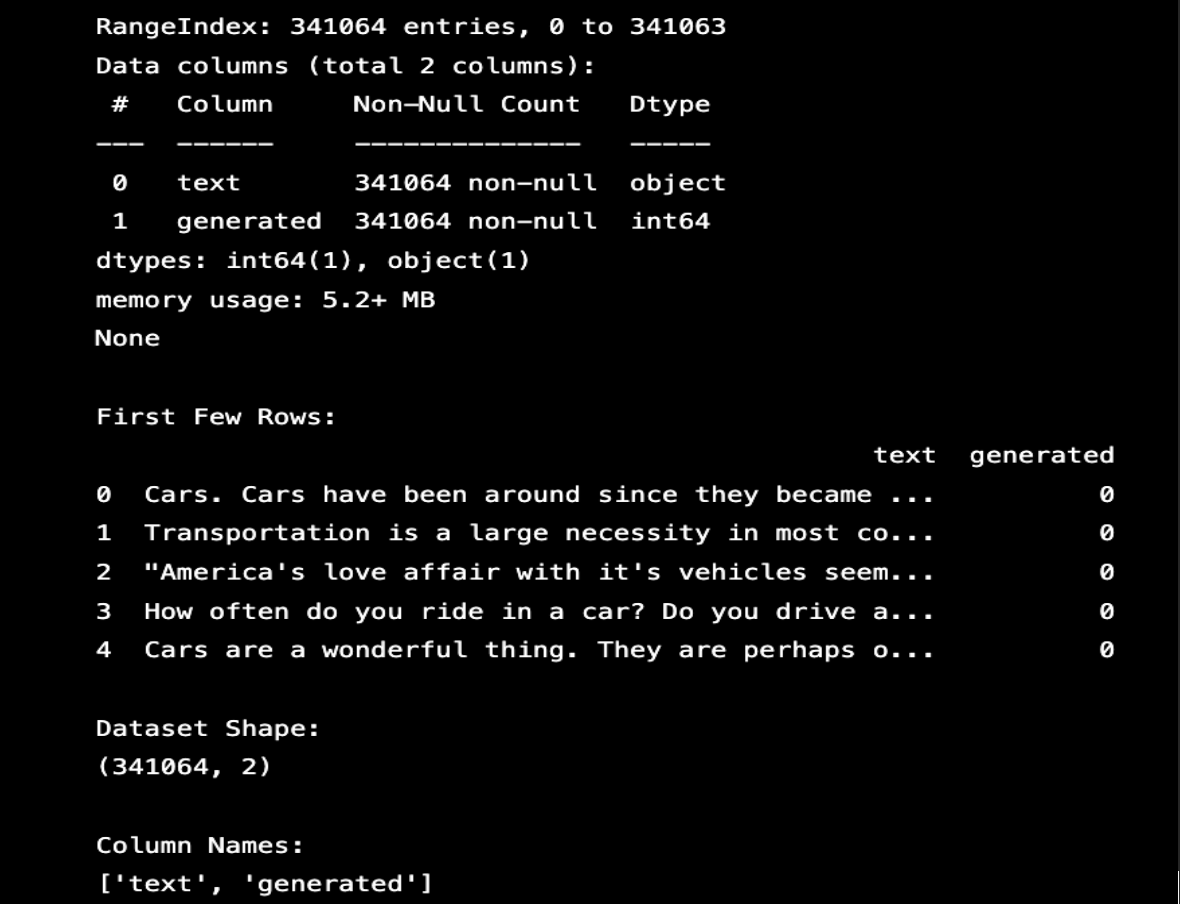
\includegraphics[width=0.8\linewidth]{Fig1.png}
\end{figure}

Therefore, the dataset at hand was of substantial size and complexity  

 
Subsequently, to establish a baseline for performance, we proceeded to train a suite of standard classifiers on the dataset. This ensemble included Logistic Regression, Naive Bayes, Decision Trees, Extra Trees Classifier, and Random Forests. Each model was rigorously evaluated using a variety of metrics, namely accuracy, precision, recall, and the F1 score, to ensure a holistic assessment of their performance. 

\begin{figure}[htbp]
  \centering
  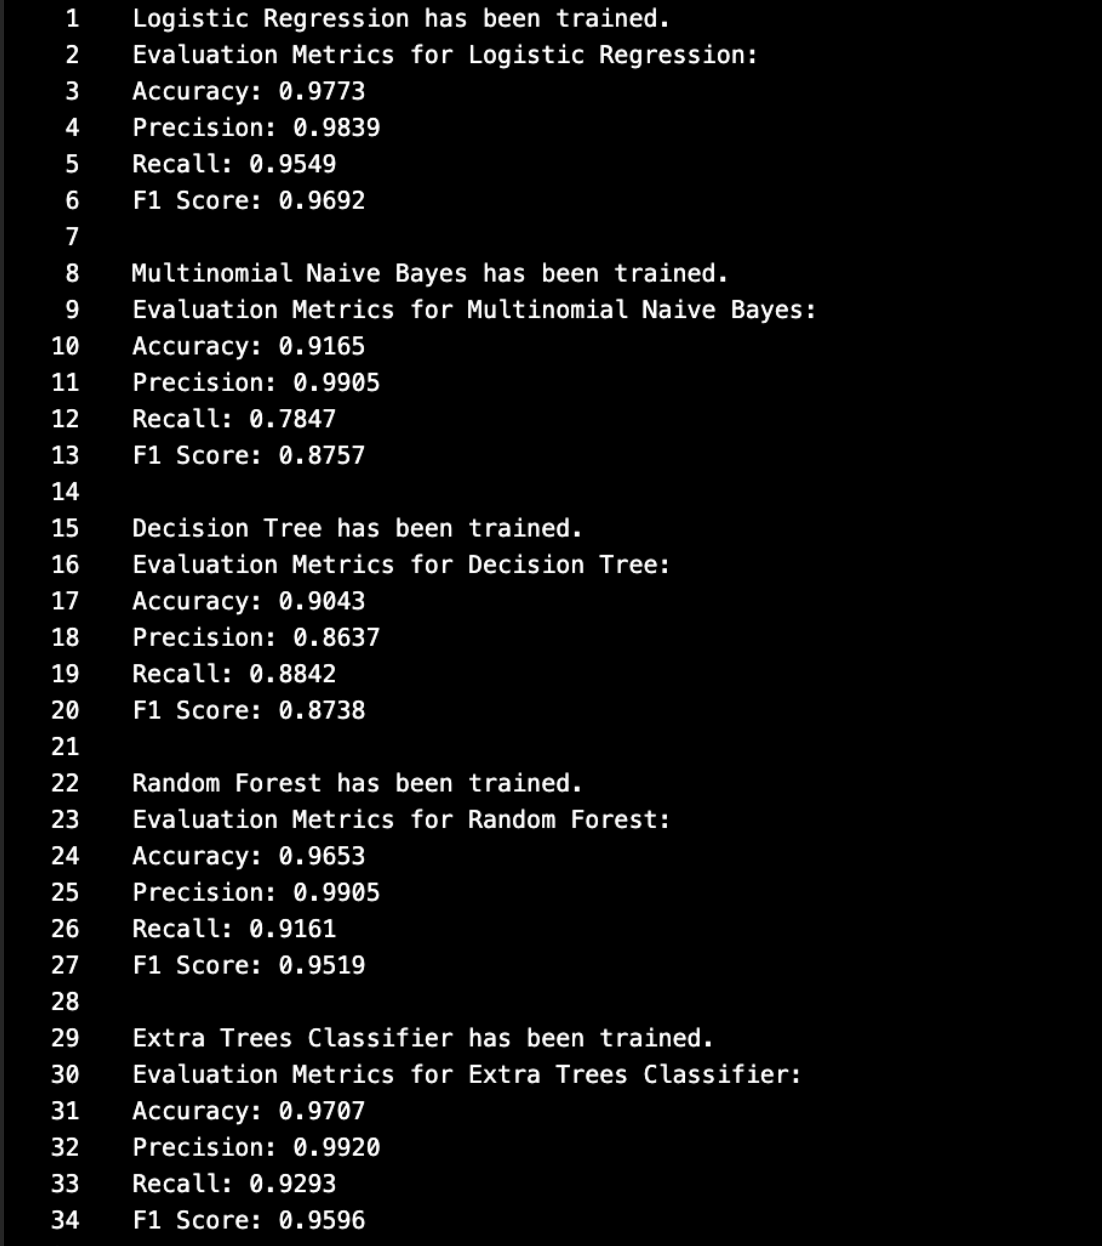
\includegraphics[width=0.8\linewidth]{Fig2.png}
\end{figure}
The results of our evaluation indicate that Logistic Regression emerged as the most effective model, demonstrating the highest levels of accuracy and F1 score among the classifiers tested. This was closely followed by the Extra Trees Classifier, which also exhibited commendable performance metrics.This structured approach not only allowed us to gauge the baseline performance of conventional classifiers on the dataset but also provided invaluable insights into the comparative efficacy of these models in handling the data's inherent complexities. 

We then proceeded to train a Long Short-Term Memory (LSTM) network 

\begin{figure}[htbp]
  \centering
  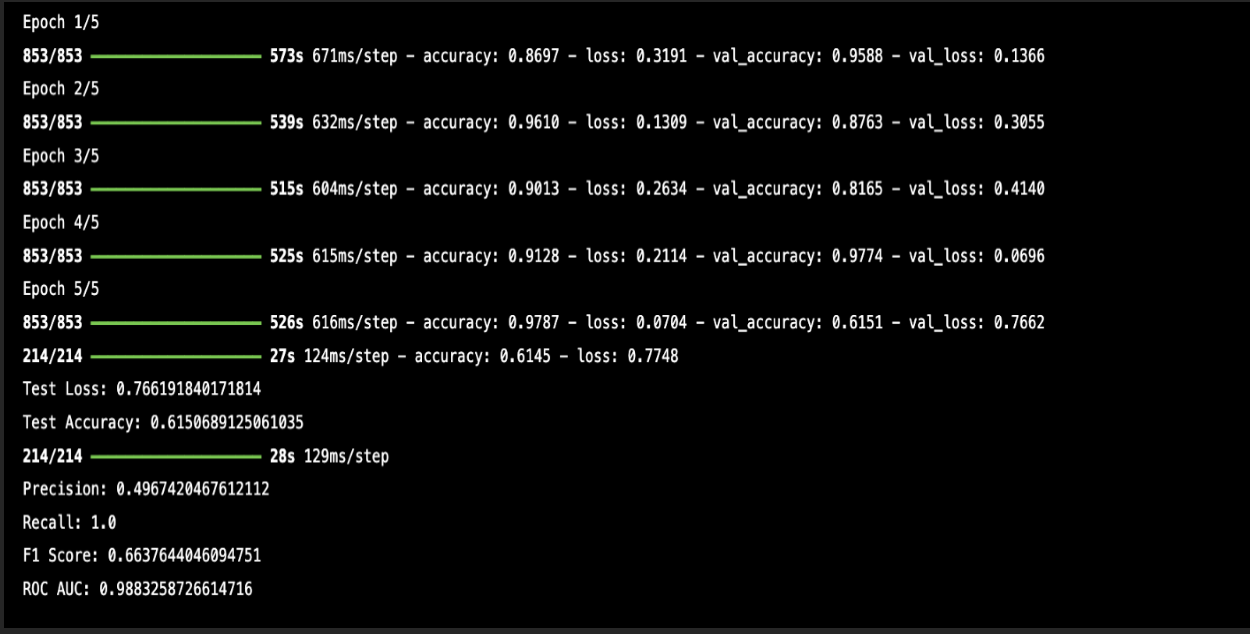
\includegraphics[width=0.8\linewidth]{Fig3.png}
\end{figure}

The model achieved a test accuracy of 61.5.The test loss stood at 0.766. Furthermore, the model demonstrated a F1 score of 0.6637 

\section{Related Work}

\textit{DetectGPT: Zero-Shot Machine-Generated Text Detection using Probability Curvature} by Eric Mitchell, Yoonho Lee, Alexander (Sasha) Khazatsky, Christopher D. Manning, and Chelsea Finn. This work focuses on computing log-probabilities in text to determine its AI-generated nature, avoiding the traditional data collection and classifier training approaches.

\textit{Real or Fake? Learning to Discriminate Machine from Human Generated Text} by Anton Bakhtin, Sam Gross, Myle Ott, Yuntian Deng, Marc'Aurelio Ranzato, and Arthur Szlam. This study leverages various machine learning models to differentiate AI-generated text, echoing the methodologies we have employed.

\textit{ChatGPT or Human? Detect and explain. Explaining Decisions of Machine Learning Model for Detecting Short ChatGPT-generated Text} by Sandra Mitrović, Davide Andreoletti, and Omran Ayoub. Utilizing a transformer-based model, this research examines the intricacies of distinguishing short AI-generated online reviews.

\textit{MGTBench: Benchmarking Machine-Generated Text Detection} by Xinlei He, Xinyue Shen, Zeyuan Chen, Michael Backes, and Yang Zhang. The introduction of MGTBench, a framework aimed at detecting machine-generated texts against advanced language models, aligns with our objectives of evaluating our model within a structured benchmark.


\section{Division of Labor}
There remain substantial areas for potential improvement and approaches that we intend to explore. Before proceeding with these directional shifts and the implementation of new ideas, we will seek guidance and insights from Dr. Culotta. 

To facilitate effective collaboration and ensure the continuity of our project's momentum, we have scheduled bi-weekly in-person meetings. Additionally, to enhance our workflow and project management, we will utilize shared Google Docs for real-time collaboration and maintain an ongoing dialogue through a dedicated group chat. This will enable us to coordinate our efforts seamlessly. 

Task allocation will be conducted with a focus on fairness and aligning responsibilities with individual interests and expertise, ensuring that both of us are engaged and contributing optimally to our collective objectives. 

\section{Timeline}
This is a guiding framework for our project's key milestones, as we do not have  precise submission dates as of yet:  
April 9th, Tuesday: Engage in a comprehensive discussion with Dr. Culotta to establish a clearly defined project direction, including the formulation of a detailed outline and plan.  
April 19th: Completion of the project report.  
April 20th: Finalize and publish the repository's README.md file. 
April 25th: Presentation of the project demo 
April 30th: Delivery of the project presentation. 

\section{References}

\bibliography{references}
\bibliographystyle{acl_natbib}
\nocite{mitchell2023detectgpt}
\nocite{bakhtin2020realorfake}
\nocite{mitrovic2023chatgpt}
\nocite{he2023mgtbench}

\end{document}
